% Template by David Madras, inspired by Meltem Atay's template for the 2018 SOCML

\documentclass{article}
\usepackage{enumitem}
\usepackage{dsfont}
\usepackage{amsmath}
\usepackage{amsfonts}
\usepackage{graphicx}
\usepackage{hyperref}
\title{Disentangling $\beta$-Variational Autoencoders}
\author{Jacob Yeung}
\date{August 28, 2020}

\begin{document}

\maketitle

My notes from the preprint Understanding disentangling in $\beta$-VAE.

\section{Background}
Altering the effect of KL divergence ($D_{KL}$) on a VAE model changes the latent features the VAE decodes. The original objective does not allow for manual alteration of the $D_{KL}$ term's effect.
\begin{equation}\label{original ELBO}
    \mathcal{L}= \mathbb{E}_{q(z|x)}p(x|z) -D_{KL}(q(z|x)\parallel p(z))
\end{equation}
Therefore to methodically explore this phenomenon, we introduce a new training objective for the variational lower bound (ELBO).
\begin{equation}\label{ELBO w/o C}
    \mathcal{L}= \mathbb{E}_{q(z|x)}p(x|z) -\beta D_{KL}(q(z|x)\parallel p(z))
\end{equation}
The original VAE model has $\beta=1$. Values of $\beta > 1$ lead to more disentangled, or factorised, latent representations, where we define disentanglement as the specificity of the learned latent feature. For example, a highly factorised feature can be the $x$-coordinate, size, or rotation of an object. Thus, single latent neurons respond only to specific single feature changes and is not affected by changes of other features. $\beta$-VAE is an unsupervised learning technique. Currently uncertain, but this could be because an increased pressure to match unit Gaussian decreases the information capacity of neurons. Fundamentally, a higher $\beta$ means increased factorization but decreased reconstruction fidelity because we are decreasing the amount of data passed through the bottleneck.

\section{Understanding Disentangling}
\subsection{Disentangling through Information Bottleneck}
We can treat the $D_{KL}$ as an upper bound of information capacity. We can minimize $D_{KL}$ by increasing the variance or decreasing the spread of the means, bringing them closer to 0. By decreasing $D_{KL}$, we are forcing the latent distributions to become similar.
\begin{center}
    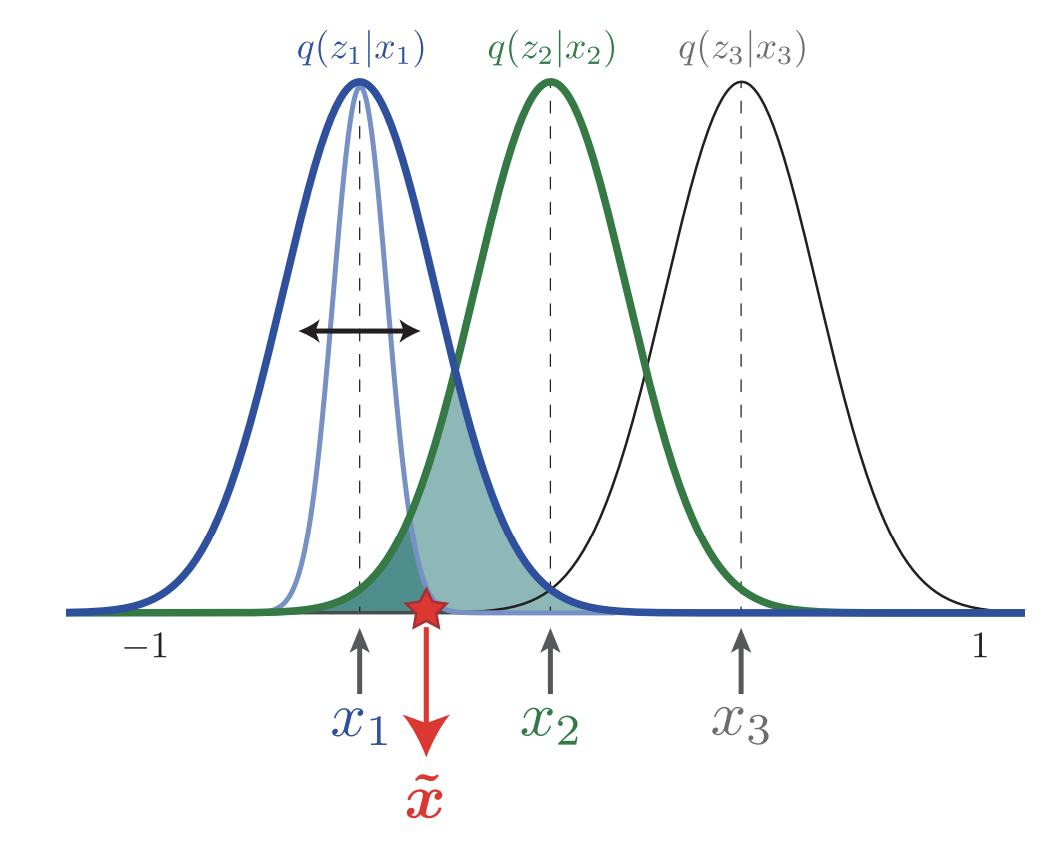
\includegraphics[width=0.75\textwidth]{DKL_as_bottleneck}
    \caption{Source:$~$Understanding disentangling in $\beta$-VAE}
\end{center}
A consequence of decreasing $D_{KL}$ is that a data point $\tilde{x}$ sampled from $q(z_1|x_1)$ can have a higher log probability of coming from $q(z_2|x_2)$ as shown in the figure. Intuitively, as posterior distributions $q_i$ overlap, they represent the same feature so there is less variance overall in the information.

\subsection{$\beta$-VAE Optimization}
Suppose a complete information bottleneck with $\beta\gg1$. Then the optimal solution is to only learn features with the largest gains in the log likelihood term.
\begin{equation}
    \mathbb{E}_{q(z|x)}p(x|z)
\end{equation}
For example, in the dSprites data set used, the different latent features span position, scale, rotation, and more. Consequently, we can see how position would yield the largest gains since if the sprites are only a few pixels off, the whole likelihood vanishes. As we increase the data bottleneck, we can focus on larger features such as scale and rotation.

\section{Methods}
\subsection{Testing Effect of Information Bottleneck}
In order to systematically test different bottlenecks, we modify our ELBO equation to the following 
\begin{equation}
    \mathcal{L}= \mathbb{E}_{q(z|f)}p(x|z) -\gamma|D_{KL}(q(z|f)\parallel p(z))-C|
\end{equation}
where $f$ are the ground truth factors, $C$ is the value we are pressuring $D_{KL}$ to become and $\gamma$ controls the amount we penalize deviation from $C$. Intuitively, at low $C$ we cannot code much information so we only focus on position latent features and as $C$ increases, the model captures more detailed variations. Note that as the information cap increases, factors of different variations are added without negatively impacting the factorization of previously learned factors.
\subsection{Application to $\beta$-VAE}
We now generalize the training model to allow the decoding net to create the factors.
\begin{equation}
    \mathcal{L}= \mathbb{E}_{q(z|x)}p(x|z) -\gamma|D_{KL}(q(z|x)\parallel p(z))-C|
\end{equation}
After obtaining the features learned at different values of $D_{KL}$ we can traverse over the features by altering the log likelihood, as shown below.
\begin{center}
    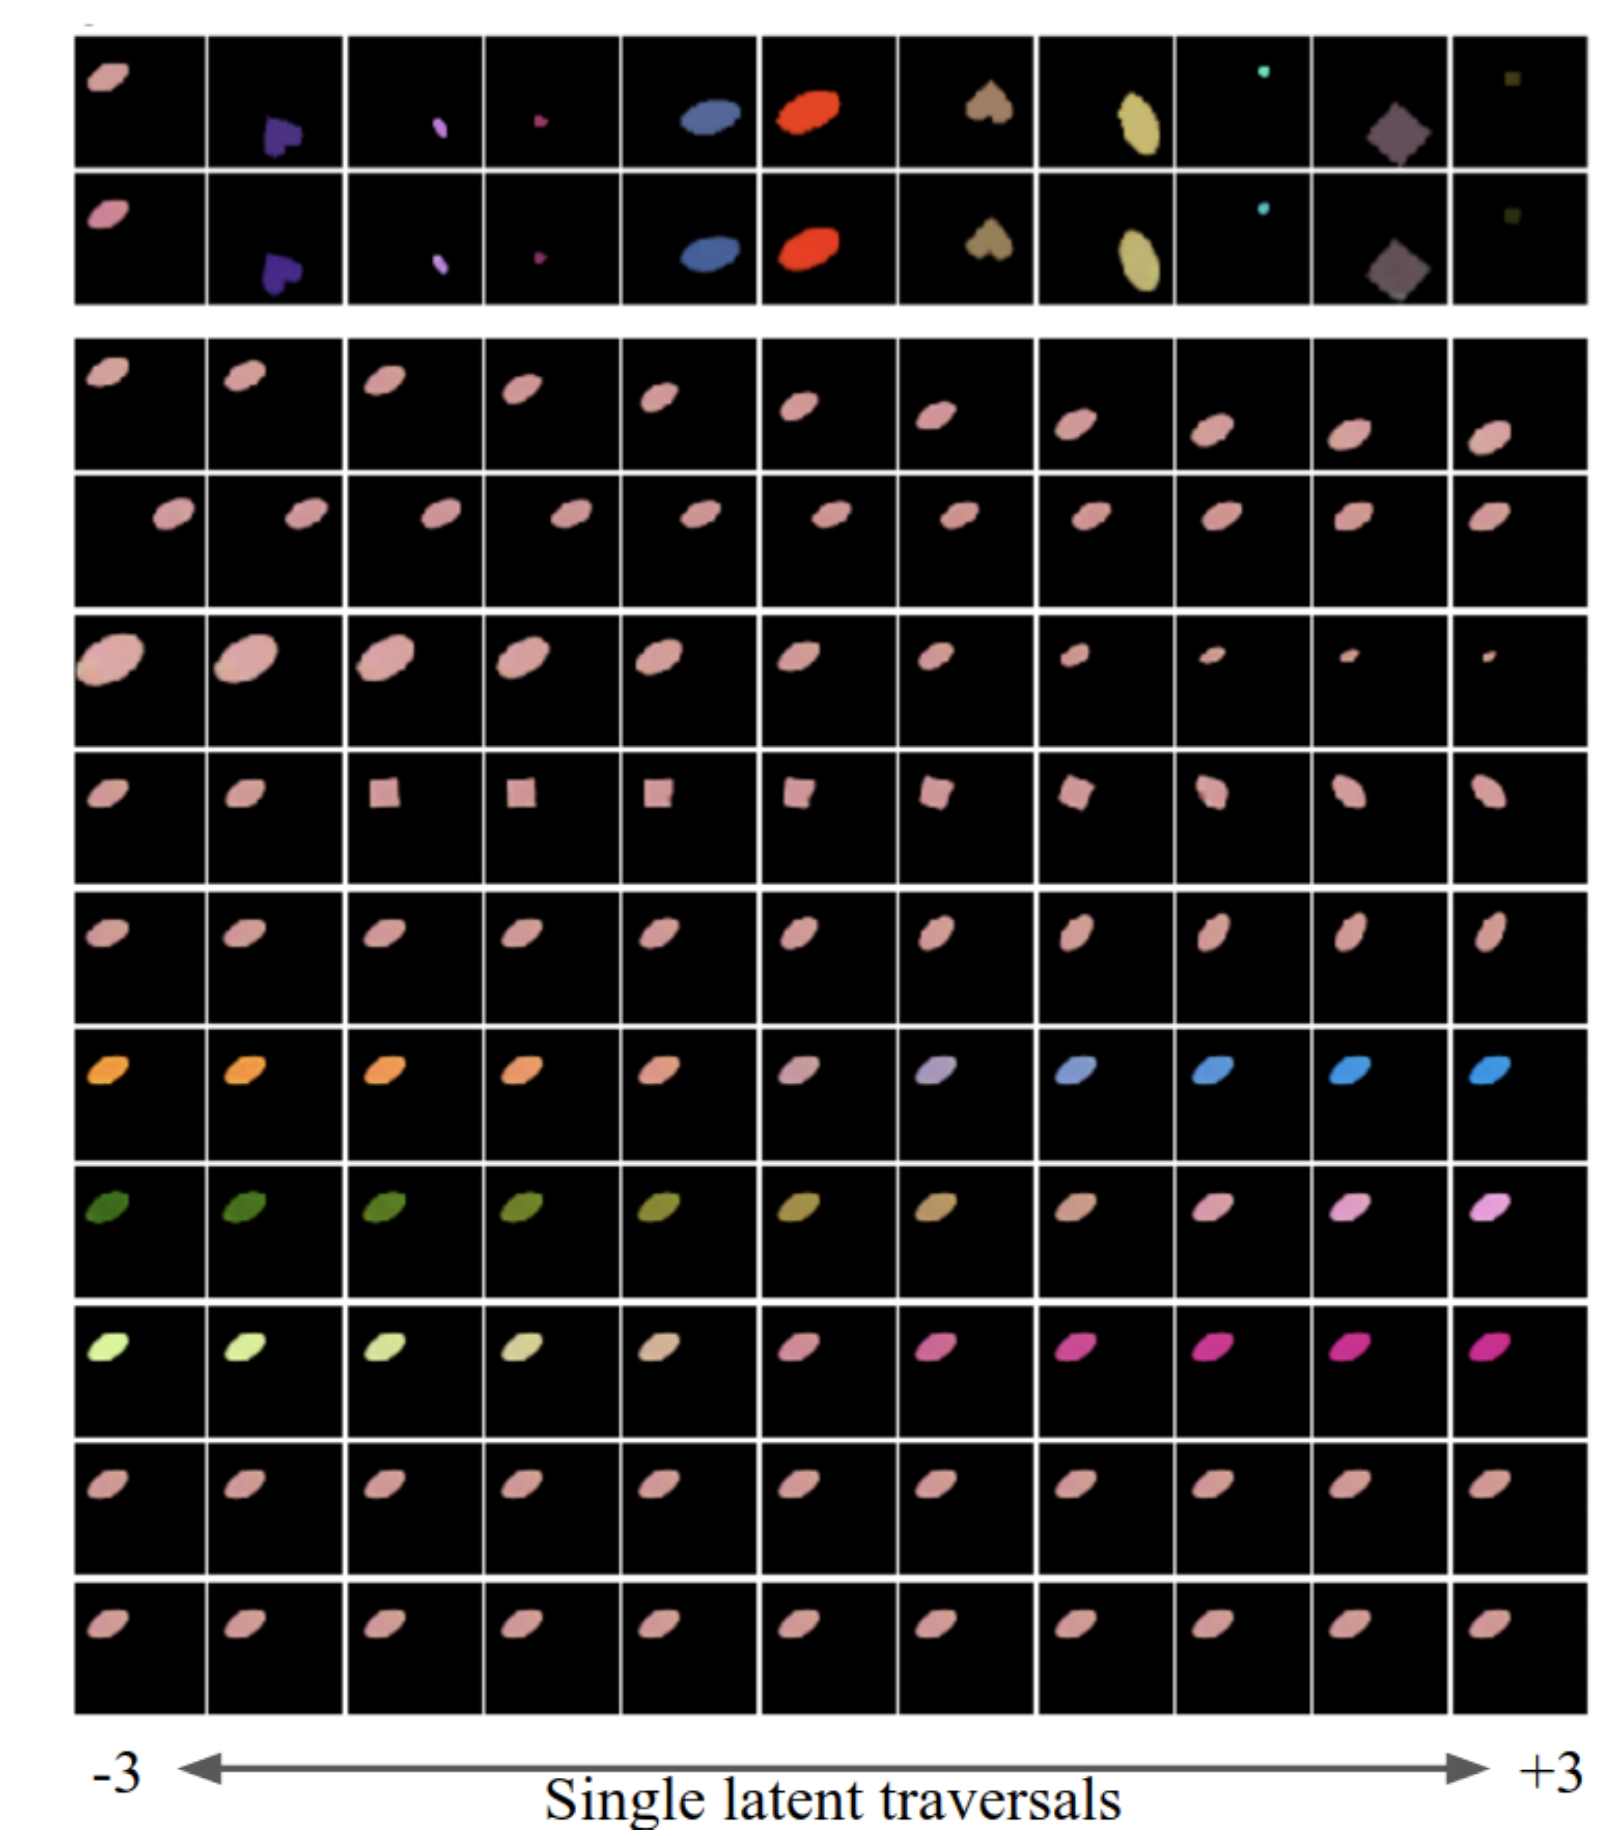
\includegraphics[width=0.75\textwidth]{reconstructions}
    \caption{Source:$~$Understanding disentangling in $\beta$-VAE}
\end{center}
The top two rows show the input and output of the model. We observe there are different latent features learned at different $D_{KL}$ values, which are ordered from high to low. At the lowest information bottleneck, we observe the model codes the latent feature for $y$-coordinate. As we decrease $D_{KL}$, the latent features code for more complex features such as rotation and color. As $D_{KL}$ approaches $0$, the latent features code for nothing.

\section{Preprint Used}
Understanding disentangling in $\beta$-VAE \href{https://arxiv.org/pdf/1804.03599.pdf}{(URL)} 
\end{document}
